\documentclass[hyperref=colorlinks]{beamer}
\mode<presentation>
\usetheme{iclpt}
\setbeamertemplate{navigation symbols}{}
\setbeamertemplate{headline}{
\begin{beamercolorbox}[leftskip=.2cm,rightskip=.2cm,topskip=.2cm,ht=1.1cm,dp=0.1cm,wd=\textwidth]{institute in head/foot}
  
\includegraphics[height=1cm]{icl.pdf}
  \hfill
  
\includegraphics[height=1cm]{../Pics/CMS-Color.pdf}
\end{beamercolorbox}
}
\setbeamertemplate{footline}{
\begin{beamercolorbox}[ht=.55cm,dp=0.4cm,wd=\textwidth,leftskip=.3cm]{author in head/foot}%
  \begin{minipage}[c]{5cm}%
    \usebeamerfont{author in head/foot}
    \insertshortauthor 
    \insertshorttitle
    \end{minipage}\hfill%
  \insertframenumber{} / \pageref{lastframe}
  \hfill
  \begin{minipage}{6cm}
    \hfill
  \end{minipage}
\end{beamercolorbox}%
}

\usepackage{color}
\usepackage{tabularx,colortbl}
\usepackage{graphicx}
\usepackage{pdfpages}
\usepackage{feynmp}
\DeclareGraphicsRule{*}{mps}{*}{}

\title{\vspace{-0.2cm} New Framework Overview}
%\subtitle{Paper - HIG-13-030, PASs: HIG-13-013, HIG-13-018, HIG-13-028 \vspace{-0.7cm}}
\author[P. Dunne]{\underline{P. Dunne} }%\\ on behalf of the H$\rightarrow$invisible analysis groups} % A.M. Magnan and A. Nikitenko Joao Pela with \\ R. Aggleton, J. Brooke: Bristol \\ C.Asawangtrakuldee, Q.Li: Peking \\ P. Srimanobhas: Chulalongkorn \\ S. Kumar, K. Mazumdar: Mumbai}
\titlegraphic{
  \vspace{-0.7cm}
  %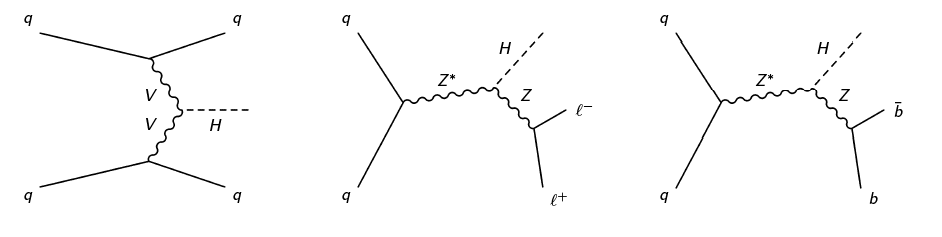
\includegraphics[width=\textwidth]{TalkPics/invcomb021213/feyndiags}
%% \begin{fmfgraph*}(100,70)
%%         \fmfleft{i1,i2}
%%         \fmfright{o1,o2,o3}
%%         \fmf{fermion}{i1,v1,o1}
%%         \fmf{fermion}{i2,v2,o3}
%%         \fmf{phantom,tension=4/5}{v1,v2}
%%         \fmffreeze
%%         \fmf{photon,label=$W,,Z$}{v1,v3}
%%         \fmf{photon,label=$W,,Z$}{v2,v3}
%%         \fmf{dashes}{v3,o2}
%%         \fmflabel{$q$}{i1}
%%         \fmflabel{$q$}{i2}
%%         \fmflabel{$q$}{o1}
%%         \fmflabel{$q$}{o3}
%%         \fmflabel{$H$}{o2}
%%       \end{fmfgraph*}
}
\date{}
\begin{document}
\begin{fmffile}{hig1330approvalfeynmandiags}

%TITLE PAGE
\section{Title}
\begin{frame}
  \titlepage
  
\end{frame}

%OUTLINE
\begin{frame}
  \frametitle{Overview}
  \begin{block}{}
    \scriptsize
    \begin{itemize}
    \item Compare updated W background estimates from both frameworks
    \item List changes since last week
    \item Twiki with instructions to have a go yourself can be found \href{https://twiki.cern.ch/twiki/bin/viewauth/CMS/VBFHinvisibleParkedData}{here}
    \end{itemize}
  \end{block}
\end{frame}

\begin{frame}
  \frametitle{Checks of framework}
  \begin{columns}
    \column{1.1\textwidth}
  \begin{block}{}
    \scriptsize
    \begin{itemize}
    \item $W\rightarrow\mu/e\nu$ background estimate module was producing slightly different results from old FW
    \item Unweighted results were identical to old framework
    \item Bug found in lepton weights code
    \item New weighted results are as below:
    \item[-] Note these numbers are different from those in our AN as they use the re-reco data
    \end{itemize}
    \begin{table}
      \begin{tabular}{|l||c|c||c|c|}
        \hline
        Result & Old FW munu & New FW munu & Old FW enu & New FW enu \\
        \hline
        NSMC & 123 & 123 & 124 & 124 \\
        NCMC & 371 & 371 & 113 & 113 \\
        NCData$-$NCBkg & 196 & 196 & 62 & 62 \\
        Result & 65.1 & 65.1 & 68.3 & 68.3 \\
        \hline
      \end{tabular}
    \end{table}
  \end{block}
  \end{columns}
\end{frame}

\begin{frame}
  \frametitle{Updates since last week}
  \begin{block}{}
    \begin{itemize}
    \item Light tree making part of old framework separated into its own executable
    \item[-] Much faster (less than half the time)
    \item[-] Should now be easier for new users to customise and run
    \item Configuration files and filelist parser added to light tree analyser
    \item[-] Code is now much neater and more changes can be made without recompiling
    \item Variable list adjusted to be compatible with all control regions of prompt analysis, Joao and Anne Marie's QCD pre-selection and future signal selection BDT.
    \item[-] Still open to optimization
    \end{itemize}
  \end{block}
\end{frame}

\begin{frame}
  \frametitle{Conclusions}
  \label{lastframe}

  \begin{block}{}
    \scriptsize
    \begin{itemize}
    \item New framework reproduces to results of old framework
    \item Light Ntuples will be uploaded to dcache soon
    \item[-] Last couple of data jobs are running
    \item Instruction to try it out can be found \href{https://twiki.cern.ch/twiki/bin/viewauth/CMS/VBFHinvisibleParkedData}{here}
    \end{itemize}
  \end{block}

\end{frame}

\begin{frame}
  \frametitle{Backup}
\end{frame}


\end{fmffile}
\end{document}
